{\large\section*{Теоритические вопросы}}

\begin{enumerate}
	\item \textit{В каком случае система запускает алгоритм унификации? (Как эту необходимость на формальном уровне распознает система?)}

	\qquad \textbf{Ответ}: алгоритм унификации запускается системой в случае необходимости проверить, подходит ли текущее правило в базе знаний для доказательства текущей цели.

	\item \textit{Каковы назначение и результат использования алгоритма унификации?}
	
	\qquad \textbf{Ответ}: результат алгоритма унификации представляет ответ да или нет. При ответе да результатом также является подстановка, сформированная в процессе работы алгоритма.
	
	\item \textit{Какое первое состояние резольвенты?}
	
	\qquad \textbf{Ответ}: первое состояние резольвенты представляет собой вопрос.

	\item \textit{Как меняется резольвента?}
	
	\qquad \textbf{Ответ}: при нахождении похдодящего правила для первого терма резольвенты он заменяется на тело правила.
	
	\item \textit{В каких пределах программы уникальны переменные?}
	
	\qquad \textbf{Ответ}: именованные переменные уникальны в пределах предложения, а анонимные переменные уникальны всегда.

	\item \textit{Как применяется подстановка, полученная с помощью алгоритма унификации?}
	
	\qquad \textbf{Ответ}: все переменные, содержащиеся в постановке и в термах резольвенты, заменяются в резольвенте на соответствующие значения для этих переменных.
	
	\item \textit{В каких случаях запускается механизм отката?}

	\qquad \textbf{Ответ}: механизм отката запускается в случае, когда система попадает в тупиковое состояние -- резольвента не пуста, но вся база знаний уже была просмотрена с целью подбора знания для текущей цели доказательства.
\end{enumerate}

{\large\section*{Задание}}

Создать базу знаний: <<ПРЕДКИ>>, позволяющую наиболее эффективным способом (за меньшее количество шагов, что обеспечивается меньшим количеством предложений БЗ -- правил), и используя разные варианты (примеры) одного вопроса, определить (указать: какой вопрос для какого варианта):

\begin{enumerate}[1.]
	\item по имени субъекта определить всех его бабушек,
	\item по имени субъекта определить всех его дедушек,
	\item по имени субъекта определить всех его бабушек и дедушек,
	\item по имени субъекта определить его бабушку по материнской линии,
	\item по имени субъекта определить его бабушку и дедушку по материнской линии.
\end{enumerate}

Минимизировать количество правил и количество вариантов вопросов. Использовать конъюнктивные правила и простой вопрос.

Для одного из вариантов ВОПРОСА и конкретной БЗ составить таблицу, отражающую конкретный порядок работы системы, с объяснениями:

\begin{itemize}[$\bullet$]
	\item очередная проблема на каждом шаге и метод ее решения;
	\item каково новое текущее состояние резольвенты, как получено;
	\item какие дальнейшие действия? (Запускается ли алгоритм унификации? Каких термов? Почему этих?);
	\item вывод по результатам очередного шага и дальнейшие действия.
\end{itemize}

\clearpage

{\large\section*{Текст программы}}

\begin{lstlisting}
domains
	name = symbol
	nameList = name*

predicates
	father(name, name).
	mother(name, name).

	parent(name, name).
	grandfather(name, name).
	grandmother(name, name).
	grandparent(name, name).
	
	allgrandfathers(name, nameList).
	allgrandmothers(name, nameList).
	allgrandparents(name, nameList).

	grandmothermline(name, name).
	grandparentsmline(name, name GrandmFather, name GrandMother).

clauses
	father(ivan, petya).
	father(petya, vasya).
	father(nastya, grisha).

	mother(ivan, nastya).
	mother(petya, lera).
	mother(nastya, masha).
	
	parent(X, Y) :- 	 father(X, Y); mother(X, Y).
	grandfather(X, Y) :- parent(X, Z), father(Z, Y).
	grandmother(X, Y) :- parent(X, Z), mother(Z, Y).
	grandparent(X, Y) :- parent(X, Z), parent(Z, Y).
	
	allgrandfathers(X, L) :- findall(Name, grandfather(X, Name), L).
	allgrandmothers(X, L) :- findall(Name, grandmother(X, Name), L).
	allgrandparents(X, L) :- findall(Name, grandparent(X, Name), L).
	
	grandmothermline(X, Y) 	:-      mother(X, Z), mother(Z, Y), !.
	grandparentsmline(X, GF, GM) :- mother(X, M), father(M, GF), mother(M, GM), !.

goal
	grandparentsmline(ivan, GF, GM).
\end{lstlisting}

\clearpage

{\large\section*{Порядок поиска ответа}}

Вопрос: по имени субъекта определить его бабушку по материнской линии.

\vspace*{5mm}

\begin{center}
	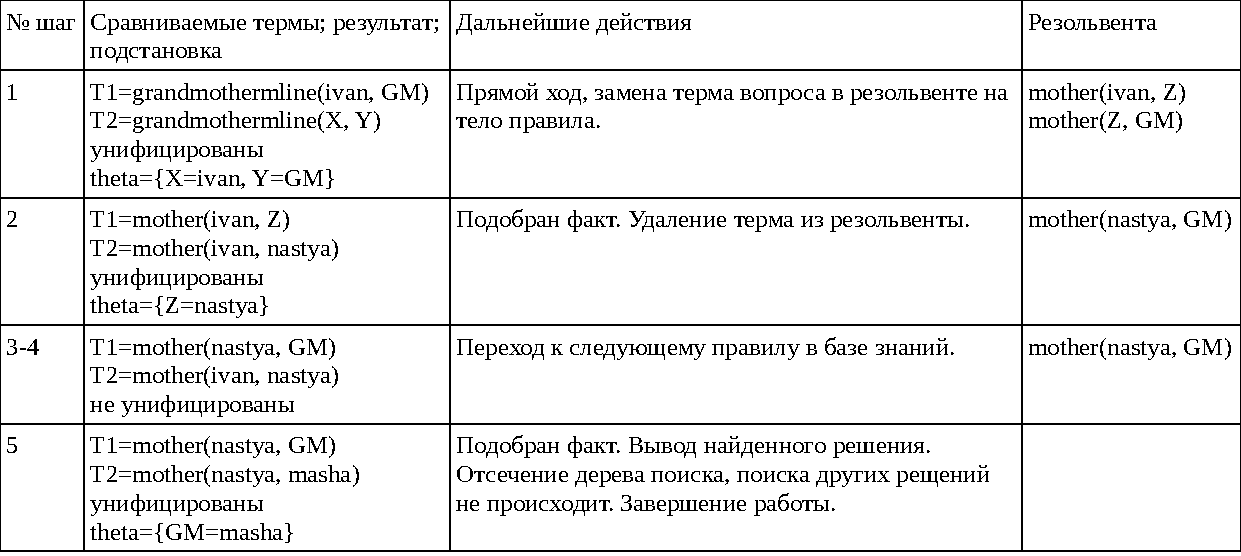
\includegraphics[width=0.95\linewidth]{table.pdf}
\end{center}
